
\section{Electric Fields and Equipotential Lines}

Name \rule{2.0in}{0.1pt}\hfill{}Section \rule{1.0in}{0.1pt}\hfill{}Date
\rule{1.0in}{0.1pt}

\textbf{Objective}

\begin{itemize}
\item To learn the shape of electric fields.
\end{itemize}
\textbf{Introduction}

Charged objects exert an electrical force on other charged objects
in proportion to the amount of charge each has, just as massive objects
exert a gravitational force on one another in proportion to their
masses. The magnitudes of both forces depend, too, on the distance
between objects. However, whereas the gravitational force is always
attractive, electrical forces may be either attractive or repulsive
depending on the sign of the charges. It is convenient in understanding
the nature of electrical forces to draw pictures of them. We represent
the fields, which provide the magnitude and direction of the forces,
as lines. We agree on a convention: the direction of the field is
that of the force on an infinitesimal positive test charge. Thus,
the lines of force originate on and come out of positive charges and
are directed toward and terminate on negative charges (see figure
below). The magnitude of the field, and therefore the force, is proportional
to the density of the field lines.

\vspace{0.3cm}
{\centering 
\includegraphics{ef_equipot_lines_fig_1.eps} \par}
\vspace{0.3cm}

Please note that when the situation is electrostatic, 1) the electric
field within a metal is zero, and 2) the electric field just outside
the surface of a metal is perpendicular to the surface. If either
of these conditions were altered, then there would be an electric
current in the metal, which is not an electrostatic situation. Because
an electric field represents a force, work must be done to move a
charged object along any of the field lines. Such work is defined
to be the potential difference between the original and final points
of movement along the lines of force. On the other hand, movement
perpendicular to the field lines requires no work. Such movement is
said to be along an equipotential line.

\vspace{0.3cm}
{\centering 
\includegraphics{ef_equipot_lines_fig_2.eps} \par}
\vspace{0.3cm}

In the figure above, the electric field for a positive point charge
is shown as lines with arrows. The regions of equipotential (equipotential
lines) are shown with circles. Notice that the equipotential lines
are perpendicular to the electric field lines and that the density
of equipotential lines is proportional to the electric field strength.

Electric field lines are difficult to measure directly, but potentials
can be measured with a voltmeter. An electric field will arise in
the space surrounding two separated charged conductors. With one lead
of a voltmeter connected to one of the conductors and the other used
as a probe, the potentials can be determined (see figure below).

\vspace{0.3cm}
{\centering \resizebox*{0.9\textwidth}{!}{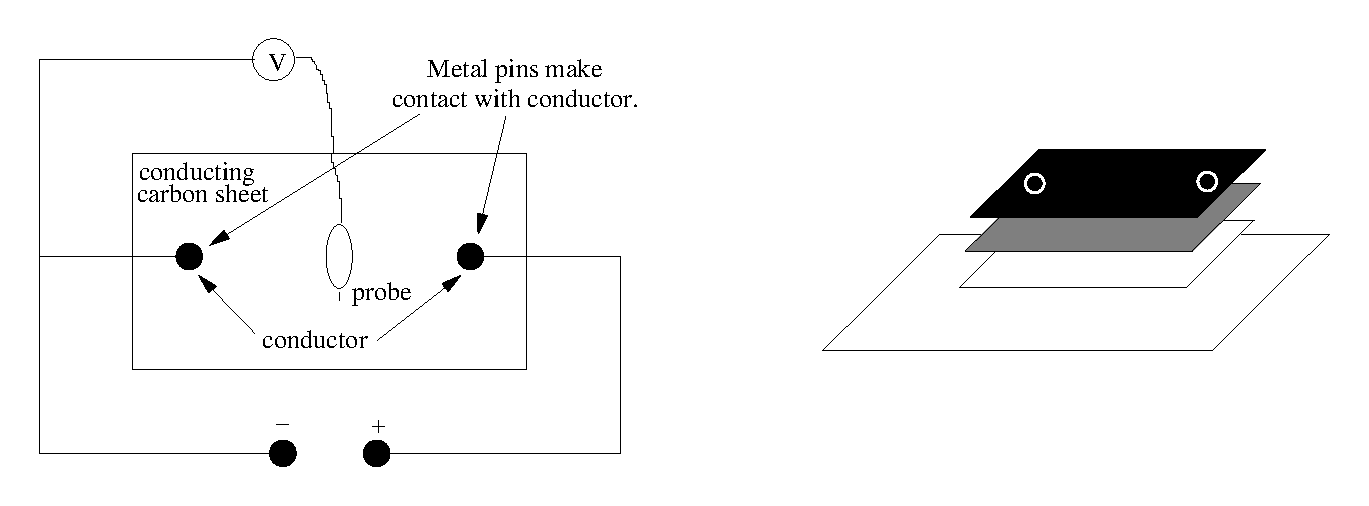
\includegraphics{ef_equipot_lines_fig_3.eps}} \par}
\vspace{0.3cm}

\textbf{Apparatus}

\begin{itemize}
\item Power supply
\item Voltmeter
\item Conducting sheets
\item Carbon and white paper
\item Wooden board and pins
\end{itemize}
\textbf{Activity 1: Field Lines for Two Point Charges}

\textbf{Prediction:} Using the rules given in the introduction and
given in the first set of figures, draw the electric lines for two
oppositely charged point objects. Sketch the equipotential lines.
\vspace{1in}

\begin{enumerate}
\item Find the conducting paper with the two silver circles on the front
and lay it over a copy carbon and a sheet of paper on top of the wooden
board.
\item Connect the positive output of the power supply to one of the circles
and the negative to the other.
\item Connect the negative lead of the voltmeter to the negative conductor
and use the positive lead as the probe. 
\item With the power supply voltage turned on and set to 10 volts, probe
lightly with the voltmeter to find a number of points on the carbon
paper registering 9 volts. Push down each time you find a point so
that marks will be made on the bottom paper.
\item Repeat for 8 volts and so on to 1 volt.
\item You should end up with a series of dots on your sheet of paper. Connect
those associated with the same potential with smooth lines.
\item Recalling the relationship between electric field lines and equipotential
lines, sketch in the electric field lines. (\emph{Other group members
can sketch copies of the same results.})
\item Does your experimental result agree with your prediction? Explain.\vspace{15mm}

\end{enumerate}
\textbf{Activity 2: Field Lines for Parallel Plates}

\textbf{Prediction:} Draw what you think the field lines and equipotential
lines between parallel plates will look like.
\vspace{1in}

\begin{enumerate}
\item Carry out the instructions from Activity 1 to check your prediction.
\item Does your result agree with your prediction? Explain.\vspace{15mm}

\end{enumerate}
\textbf{Activity 3: Field Lines Between a Point Charge and a Plate}

\textbf{Prediction:} Draw what you think the field lines and equipotential
lines between a point charge and a parallel plate will look like.
\vspace{1in}

\begin{enumerate}
\item Map the field lines as before.
\item Does your result agree with your prediction? Explain.\vspace{15mm}

\item If the potential is zero, must the electric field be zero as well?\vspace{15mm}

\item What can you say about the electric field along an equipotential line?\vspace{15mm}

\end{enumerate}
\textbf{Activity 4: Field Lines for a Plate and a Charged Circle}

\textbf{Prediction:} Sketch what you think the field and potential
lines between a charged circle and a plate look like.
\vspace{1in}

\begin{enumerate}
\item Determine the field lines.
\item What is the field strength within a charged, continuous surface?\vspace{15mm}
\end{enumerate}

